%!TEX program = xelatex
\documentclass[10pt, compress]{beamer}
\usetheme[titleprogressbar]{m}

\usepackage{booktabs}
\usepackage[scale=2]{ccicons}
\usepackage{minted}
\newcommand\myheading[1]{%
  \par\bigskip
  {\Large\bfseries#1}\par\smallskip}

\usepgfplotslibrary{dateplot}

\usemintedstyle{trac}

\title{Augmented Reality and GIS}
\subtitle{}
\author{Ockert Malan}
\institute{Presentiation as part of Scientific Computing 372 and Geo-Information Technology 341}

\begin{document}

\maketitle

\begin{frame}[fragile]
\frametitle{What is Augmented Reality?}
\myheading{What Wikipedia says:}
\textit{``Augmented Reality (AR) is an interactive experience of a real-world environment whereby the objects that reside in the real-world are 'augmented' by computer-generated perceptual information..."}
\end{frame}

\begin{frame}[fragile]
\frametitle{What is GIS?}
\myheading{What Wikipedia says:}
\textit{``A geographic information system (GIS) is a system designed to capture, store, manipulate, analyze, manage, and present spatial or geographic data."}
\end{frame}

\begin{frame}[fragile]
\frametitle{What is ARGIS?}
When these technologies are combined you end up with ARGIS.\\

But what exactly is it in practice?
\end{frame}

\begin{frame}[fragile]
  \frametitle{What is ARGIS?}
  Take for example the scene behind this wall...
\begin{figure}
  \centering
 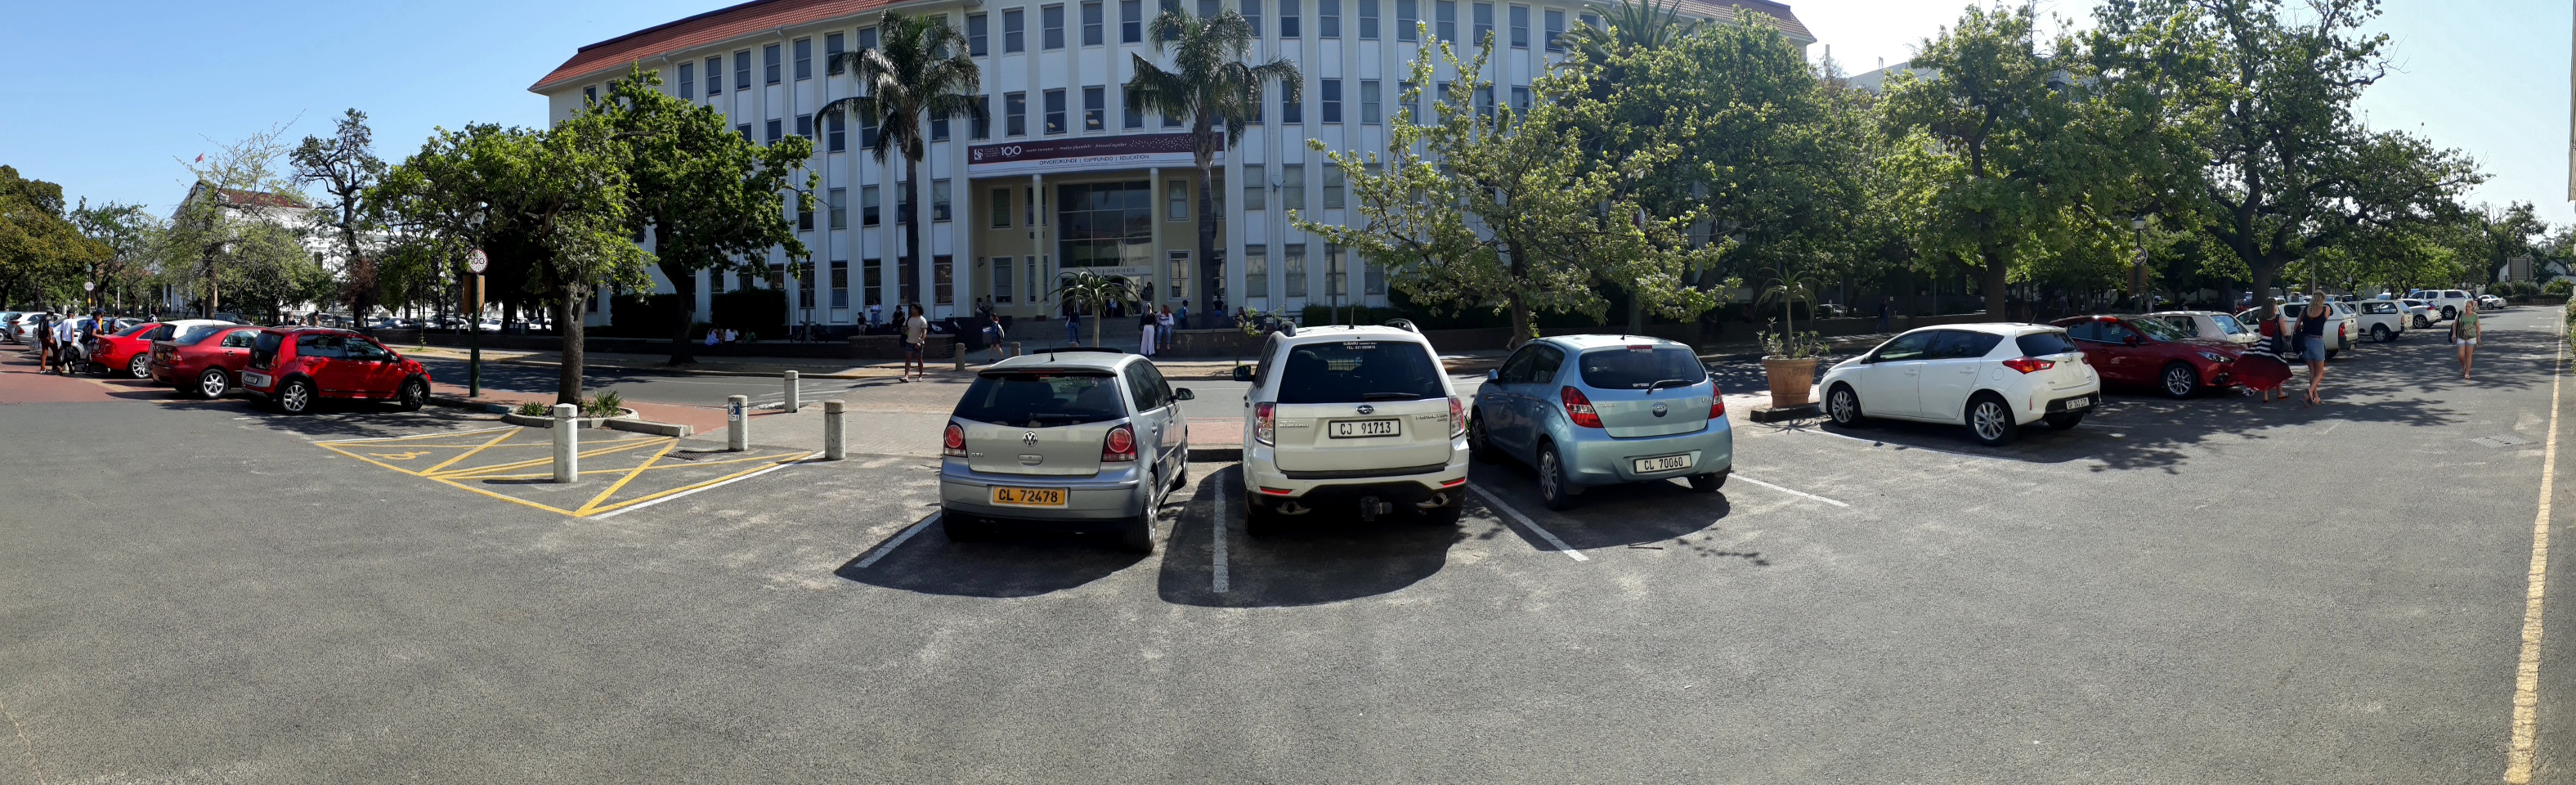
\includegraphics[width=11cm,height=3.5cm]{1.jpg}
\end{figure}
\end{frame}

\begin{frame}[fragile]
  \frametitle{What is ARGIS}
  ...as well as the spatial data that can be contained about it in a GIS.
\begin{figure}
  \centering
 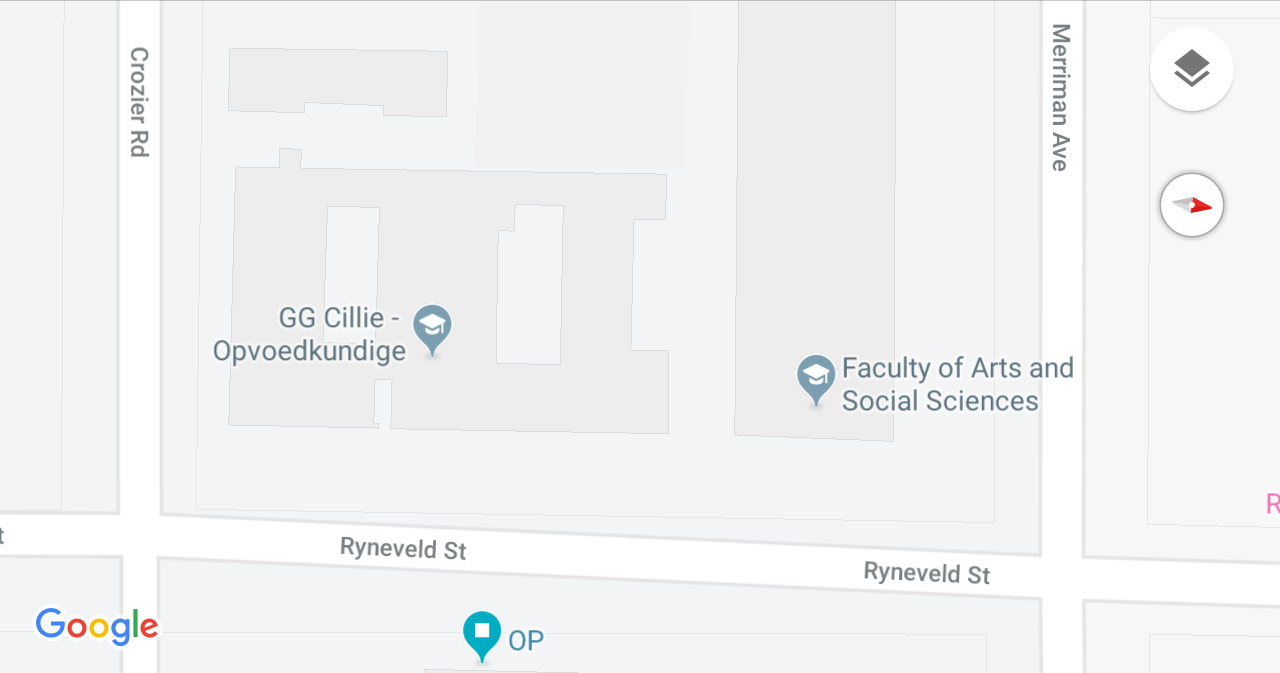
\includegraphics[width=11cm,height=5cm]{2.png}
\end{figure}
\end{frame}

\begin{frame}[fragile]
  \frametitle{What is ARGIS}
  This information can then be displayed (badly in this case) on the scene itself using AR:
\begin{figure}
  \centering
 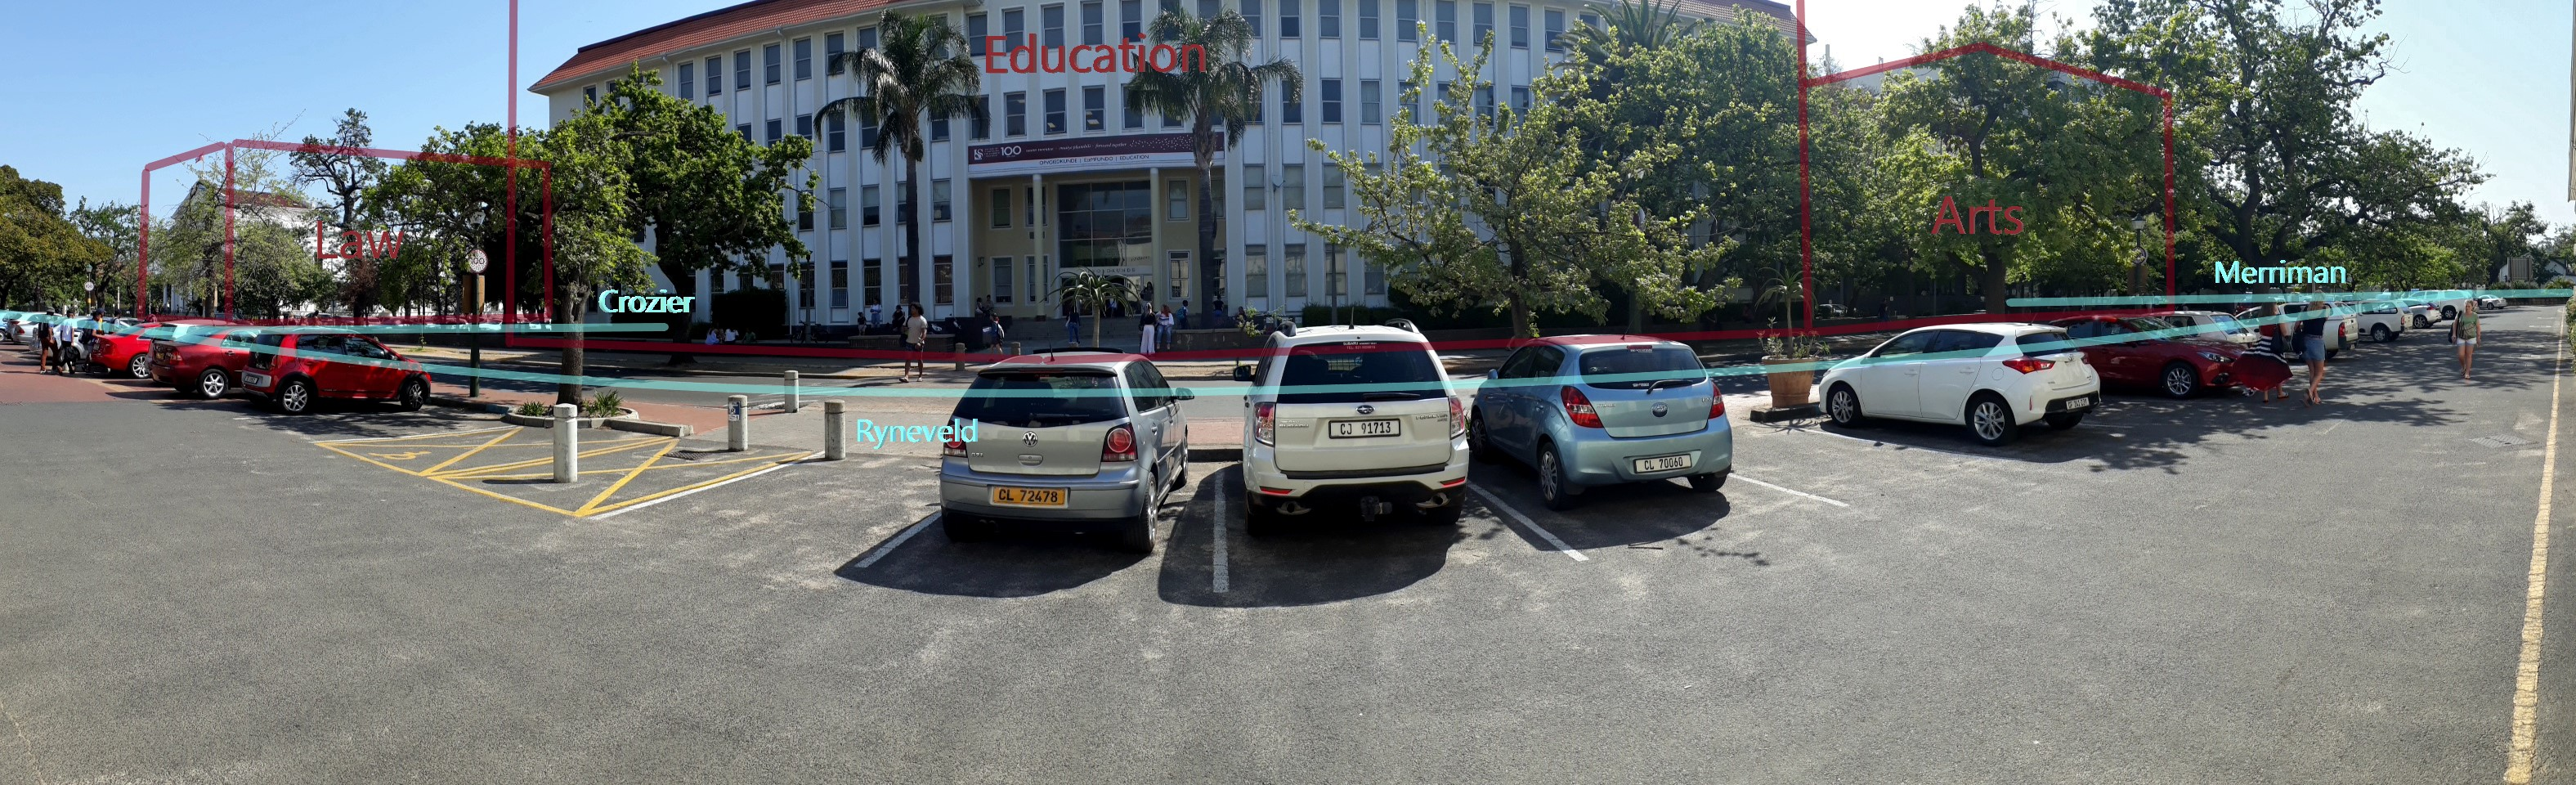
\includegraphics[width=11cm,height=3.5cm]{3.jpg}
\end{figure}
\end{frame}

\begin{frame}[fragile]
\frametitle{What is ARGIS?}
This allows for a more intuitive and user-friendly way of viewing and even interacting with Geospatial Data.

\end{frame}

\begin{frame}[fragile]
\frametitle{History of ARGIS?}
The concept of ARGIS has been around since the 1990s, but recent advances in technology have allowed for superior implementation by increasing system performance, portability and interactivity (Boulos et al, 2017).
\end{frame}

\begin{frame}[fragile]
\frametitle{Why should we care?}
\end{frame}

\begin{frame}[fragile]
\frametitle{Why should we care?}
Well ARGIS is quickly gaining traction as a way of interfacing with spatial data (Zhang et al, 2016) with both potential and proven examples:
\end{frame}

\begin{frame}[fragile]
\frametitle{Examples:}
Well ARGIS is quickly gaining traction as a way of interfacing with spatial data (Zhang et al, 2016) with both potential and proven examples:
\end{frame}

\begin{frame}[fragile]
\frametitle{References:}
Boulos, M.N.K., Lu, Z., Guerrero, P., Jennett, C. and Steed, A., 2017. From urban planning and emergency training to Pokémon Go: applications of virtual reality GIS (VRGIS) and augmented reality GIS (ARGIS) in personal, public and environmental health.\\

Zhang, X., Han, Y., Hao, D. and Lv, Z., 2016. ARGIS-based outdoor underground pipeline information system. Journal of Visual Communication and Image Representation, 40, pp.779-790.
\end{frame}

\end{document}
